\documentclass[a4paper,14pt]{extreport} % формат документа

\usepackage{amsmath}
\usepackage{cmap} % поиск в ПДФ
\usepackage[T2A]{fontenc} % кодировка
\usepackage[utf8]{inputenc} % кодировка исходного текста
\usepackage[english,russian]{babel} % локализация и переносы
\usepackage[left = 2cm, right = 1cm, top = 2cm, bottom = 2 cm]{geometry} % поля
\usepackage{listings}
\usepackage{graphicx} % для вставки рисунков
\usepackage{amsmath}
\usepackage{float}
\usepackage{multirow}
\graphicspath{{img/}}
\DeclareGraphicsExtensions{.pdf,.png,.jpg}
\newcommand{\anonsection}[1]{\section*{#1}\addcontentsline{toc}{section}{#1}}

\lstset{ %
	language=Lisp,                % Язык программирования 
	numbers=left,                   % С какой стороны нумеровать          
	frame=single,                    % Добавить рамку
}

\begin{document}
\begin{titlepage}

    \begin{table}[H]
        \centering
        \footnotesize
        \begin{tabular}{cc}
            \multirow{8}{*}{
\includegraphics[scale=0.35]{bmstu.jpg}}
            & \\
            & \\
            & \textbf{Министерство науки и высшего образования Российской Федерации} \\
            & \textbf{Федеральное государственное бюджетное образовательное учреждение} \\
            & \textbf{высшего образования} \\
            & \textbf{<<Московский государственный технический} \\
            & \textbf{университет имени Н.Э. Баумана>>} \\
            & \textbf{(МГТУ им. Н.Э. Баумана)} \\
        \end{tabular}
    \end{table}

    \vspace{-2.5cm}

    \begin{flushleft}
        \rule[-1cm]{\textwidth}{3pt}
        \rule{\textwidth}{1pt}
    \end{flushleft}

    \begin{flushleft}
        \small
        ФАКУЛЬТЕТ
        \underline{<<Информатика и системы управления>>\ \ \ \ \ \ \ 
        \ \ \ \ \ \ \ \ \ \ \ \ \ \ \ \ \ \ \ \ \ \ \ \ \ \ \ \ \ \ \ 
    \ \ \ \ \ \ \ \ \ \ \ \ \ \ \ } \\
        КАФЕДРА
        \underline{<<Программное обеспечение ЭВМ и
        информационные технологии>>
        \ \ \ \ \ \ \ \ \ \ \ \ \ \ \ \ \ \ \ \ }
    \end{flushleft}

    \vspace{2cm}

    \begin{center}
        \textbf{Лабораторная работа № 4} \\
        \vspace{0.5cm}
    \end{center}

    \vspace{4cm}

    \begin{flushleft}
        \begin{tabular}{ll}
            \textbf{Дисциплина} & Экономика программной инженерии.  \\
            \textbf{Тема} & Актуализация параметров проекта. \\
            & Ввод фактических данных для \\
            & задач и просмотр отклонений от контрольного плана \\
            \\
            \textbf{Студент} & Сусликов Д.В. \\
            \textbf{Группа} & ИУ7-85Б \\
            \textbf{Оценка (баллы)} & \\
            \textbf{Преподаватель} & Барышникова М.Ю., Силантьева А.В.   \\
        \end{tabular}
    \end{flushleft}

    \vspace{4cm}

   \begin{center}
        Москва, 2022 г.
    \end{center}

\end{titlepage}

\begin{enumerate}

\item \textbf{Основное задание}

Содержание проекта: Команда разработчиков из 16 человек занимается созданием карты города на основе собственного модуля отображения. Проект должен быть завершен в течение 6 месяцев. Бюджет проекта: 50 000 рублей.

\item \textbf{Задайте дату отчета (20 апреля).}

\begin{figure}[H]
  \centering
  \caption{Дата отчета. }
  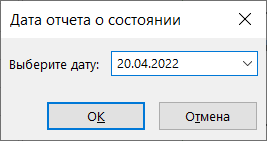
\includegraphics[scale=1.5]{1}
\end{figure}

\item \textbf{Внесите фактические данные для отдельных задач проекта (по заданию преподавателя).}

Отметить как выполненные все работы, которые должны были завершиться на эту дату, кроме:
\begin{itemize}
	\item 6 -- закончилась на неделю позже 
	\item 9 -- началась на неделю позже
	\item 14 -- ведущий программист с 1 апреля на 10 дней ушёл на повышение квалификации, после этого з/п у него выросла на 10\%
	\item 10 -- выполнена на 50\%
	\item Мультимедиа-корреспондент с 5 апреля ушёл на недельный больничный
	\item c 1 апреля на совещания назначаются только те ведущие специалисты, что работали за неделю до совещания и неделю после
\end{itemize}

\newpage

Изменяем дату окончания Задачи 6:
\begin{figure}[H]
	\centering
	\caption{Новая дата окончания Задачи 6. }
	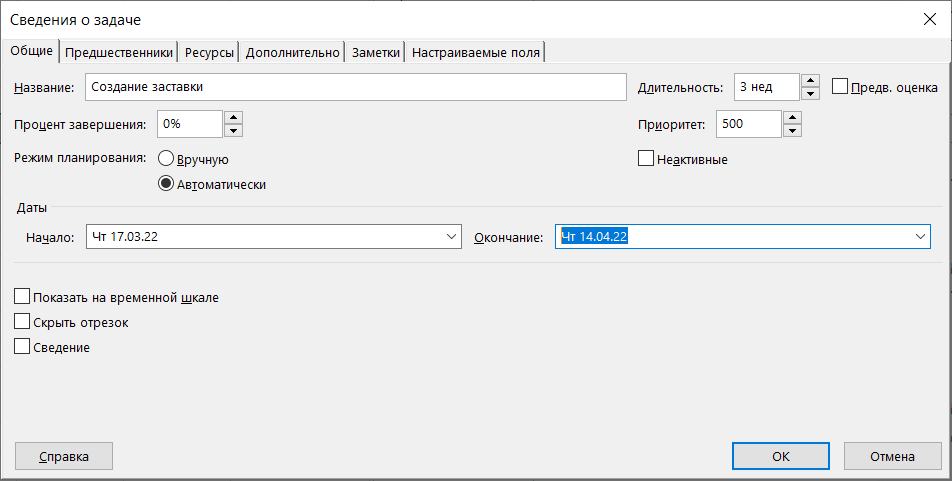
\includegraphics[scale=0.7]{delay-task6}
\end{figure}

Изменяем дату начала Задачи 9:
\begin{figure}[H]
	\centering
	\caption{Новая дата начала Задачи 9. }
	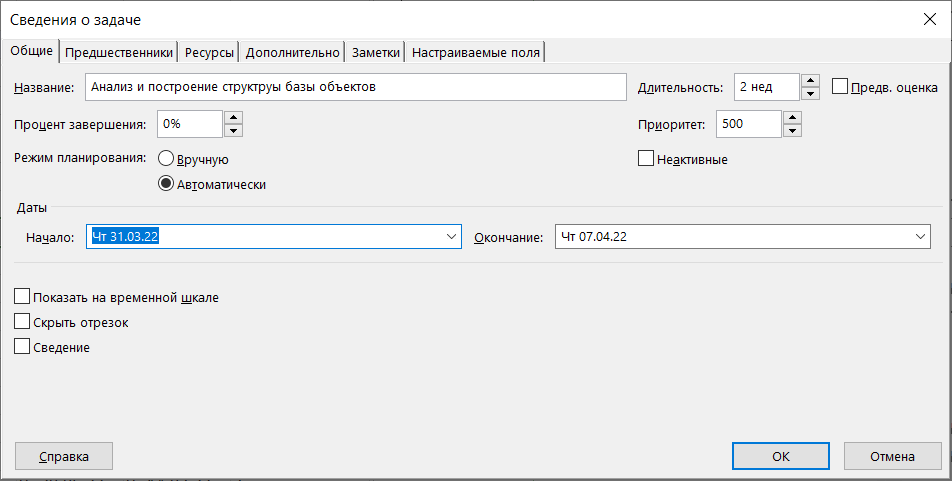
\includegraphics[scale=0.7]{delay-task9}
\end{figure}

На промежуточном результате видны переработки, которые в конце будут исправлены.
\begin{figure}[H]
	\centering
	\caption{Промежуточный результат. }
	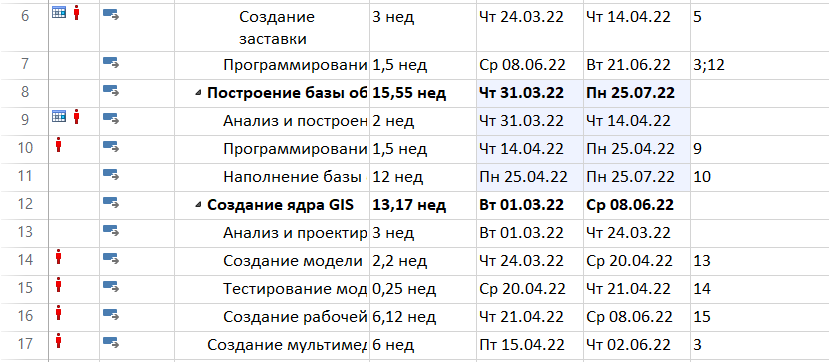
\includegraphics[scale=0.8]{delay-results}
\end{figure}

Ведущий программист с 1 апреля на 10 дней ушёл на повышение квалификации.
\begin{figure}[H]
	\centering
	\caption{Уход на повышение квалификации. }
	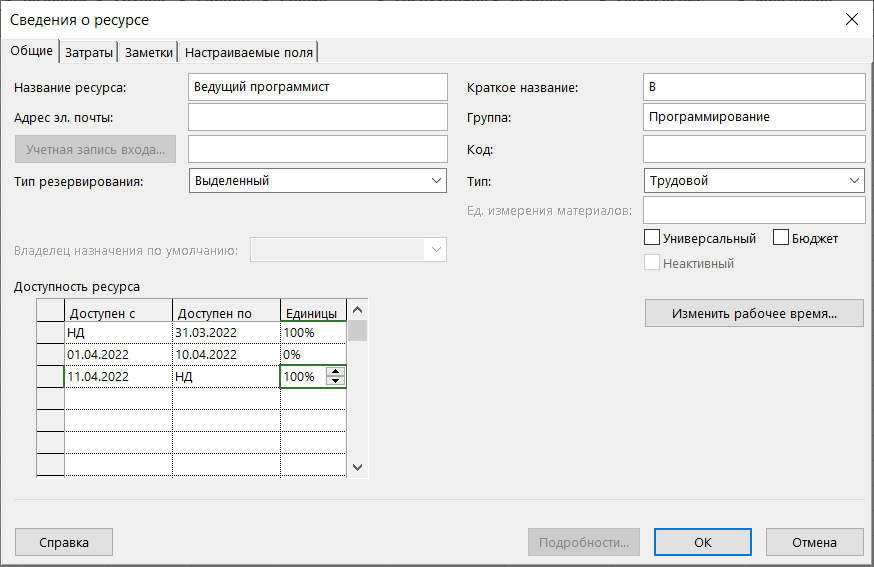
\includegraphics[scale=0.8]{powerup}
\end{figure}

Повышение з/п ведущему программисту на 10\%.
\begin{figure}[H]
	\centering
	\caption{Повышение з/п ведущему программисту. }
	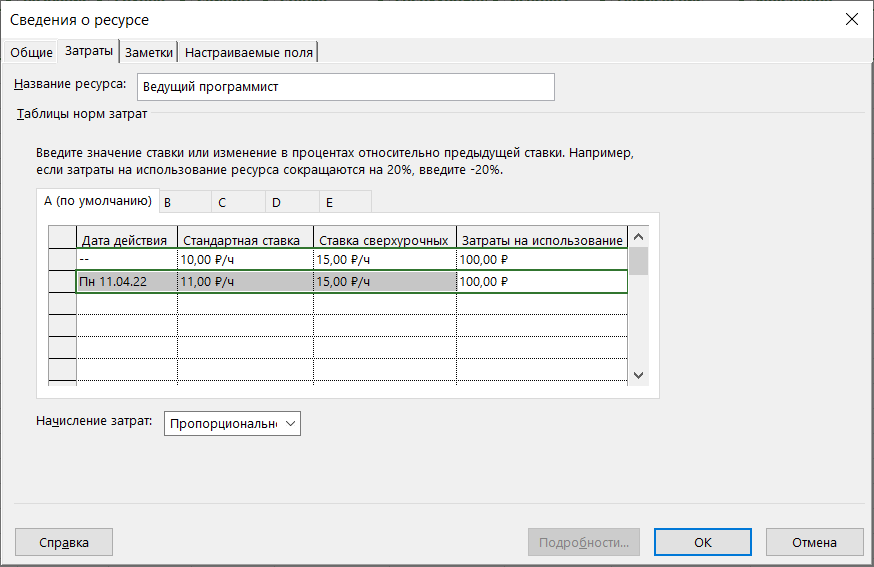
\includegraphics[scale=0.8]{powerup2}
\end{figure}

Возникает еще перегрузка для ведущего программиста, что будет ликвидирована в конце.

Отмечаем, что Задача 10 выполнена на 50\%.
\begin{figure}[H]
	\centering
	\caption{Задача 10 выполнена на половину (не выполнена на половину). }
	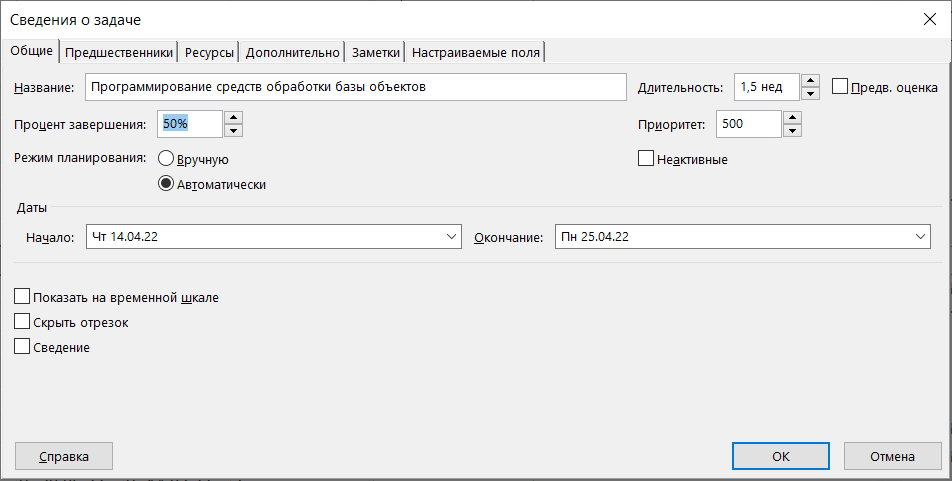
\includegraphics[scale=0.8]{task10}
\end{figure}

Мультимедиа-корреспондент с 5 апреля ушёл на недельный больничный.
\begin{figure}[H]
	\centering
	\caption{Больничный для мультимедиа-корреспондента. }
	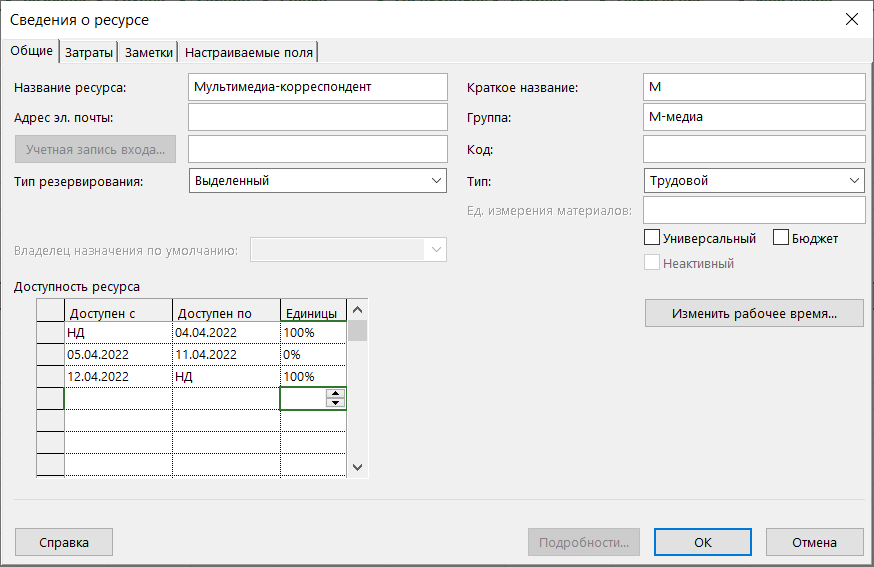
\includegraphics[scale=0.8]{chill}
\end{figure}

Убираем ненужные часы для совещаний для определенных работников и проводим выравнивания ресурсов. 

\begin{figure}[H]
	\centering
	\caption{Исключение из ненужных для сотрудника совещаний. }
	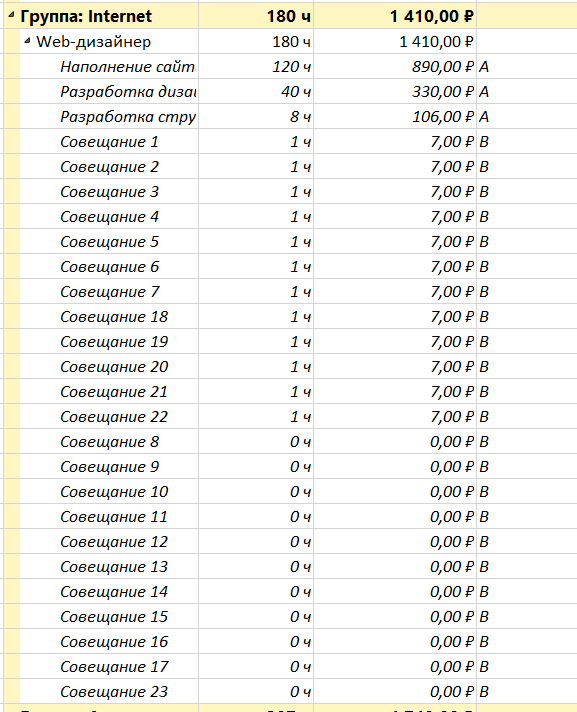
\includegraphics[scale=0.8]{meetings}
\end{figure}

После этого получаем.

\begin{figure}[H]
  \centering
  \caption{Итог после выполнения всех заданий. }
  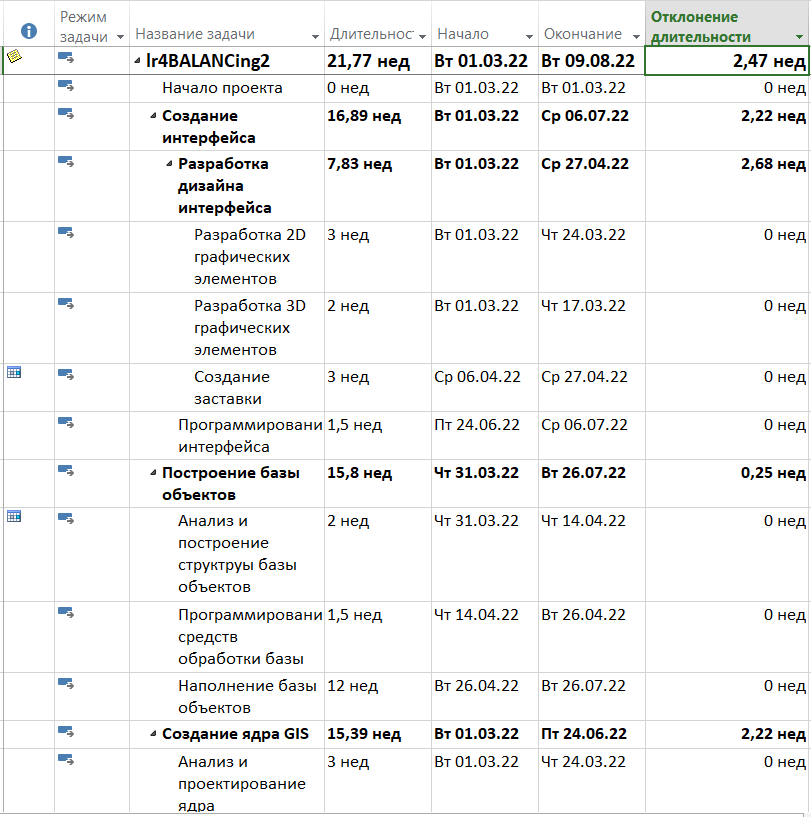
\includegraphics[scale=0.8]{result1}
\end{figure}

\begin{figure}[H]
	\centering
	\caption{Итог после выполнения всех заданий. }
	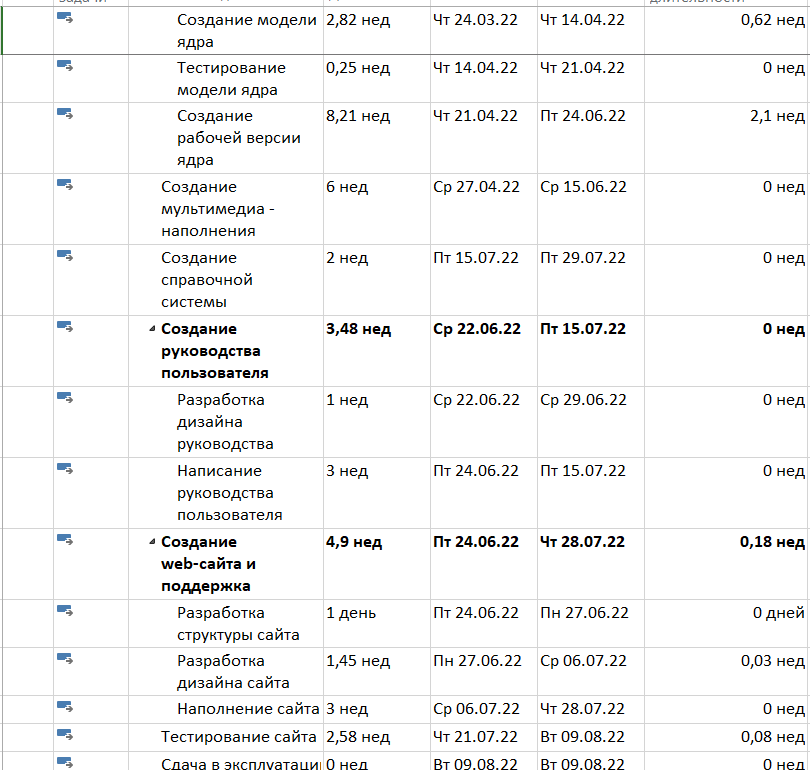
\includegraphics[scale=0.8]{result2}
\end{figure}

\begin{figure}[H]
	\centering
	\caption{Итог после выполнения всех заданий. }
	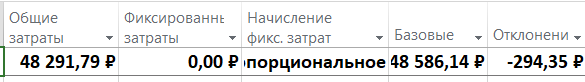
\includegraphics[scale=0.8]{result3}
\end{figure}
Срок окончания сдвигается с 27 июля на 9 августа. Затраты уменьшились с 48586,14 рублей до 48291,14.

Таким образом, хоть срок окончания сдвинулся вперед, проект все равно укладывается во временные рамки. Хоть сроки работ и увеличилсь, бюджет не увеличился, а лишь наоброт уменьшился, это связано с тем, что были убраны лишние люди с совещаний.


\end{enumerate}

\end{document}